\subsection{Законы Кеплера}
\term{I-ый закон:} Все планеты движутся по
эллиптическим орбитам, в одном из фокусов которых
находится Солнце.\\

\term{ II-ой закон:} Радиус-вектор планеты за
равные промежутки времени заметает равные площади:
\begin{equation}
	\frac{dS}{dt}=\const = \frac{S_\text{элл}}{T} = \frac{\pi a b }{T}.
\end{equation}
\term{III-ий закон:} Квадраты периодов обращения планет
относятся как кубы больших полуосей их орбит.
\begin{equation}
	\frac{T^2_1}{T^2_2}=\frac{a^3_1}{a^3_2},
\end{equation}
где $a$ --- большая полуось, $T$ --- период обращения.
\begin{figure}[h!]
	\begin{minipage}[b]{0.5\textwidth}
		\centering
		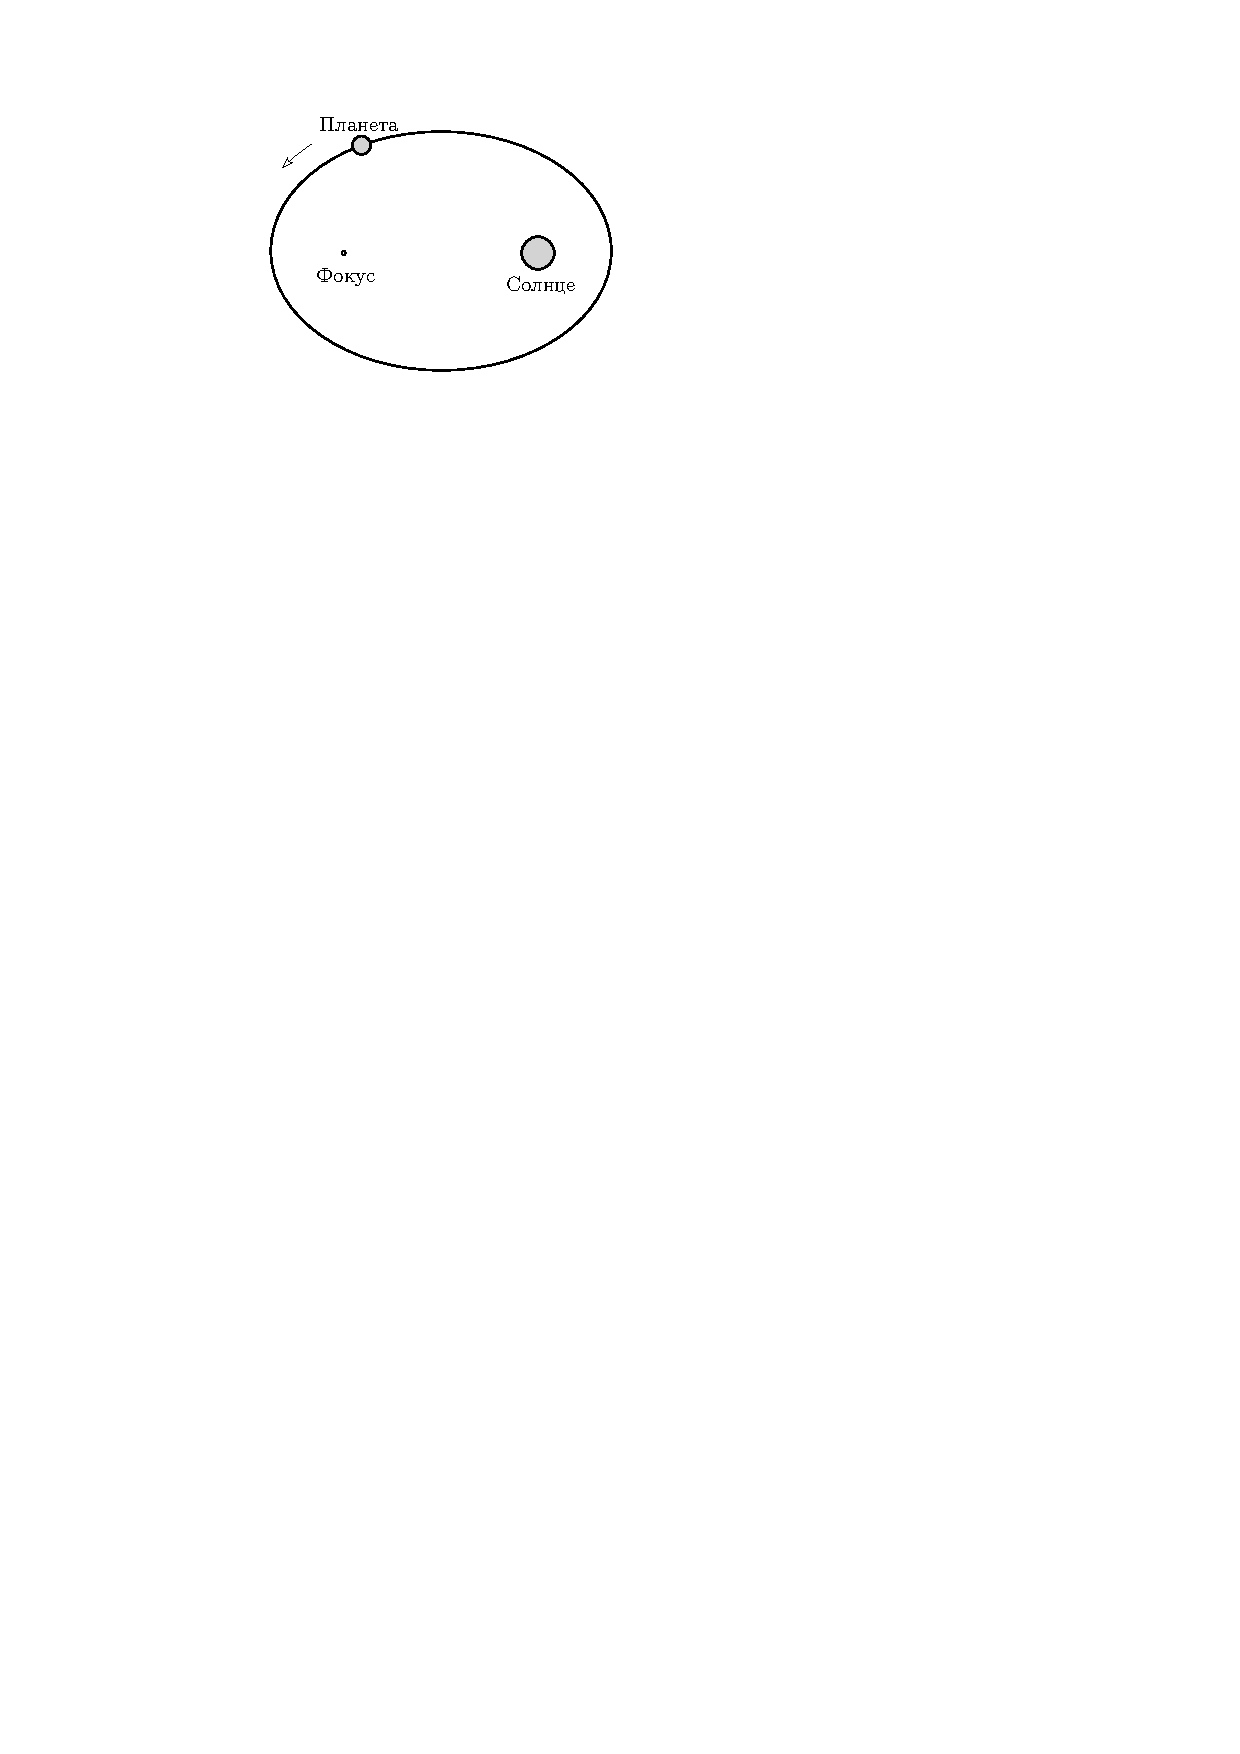
\includegraphics[width = 0.84\textwidth]{first-kepler}
		\caption{Первый закон Кеплера}
	\end{minipage}
	\begin{minipage}[b]{0.5\textwidth}
		\centering
		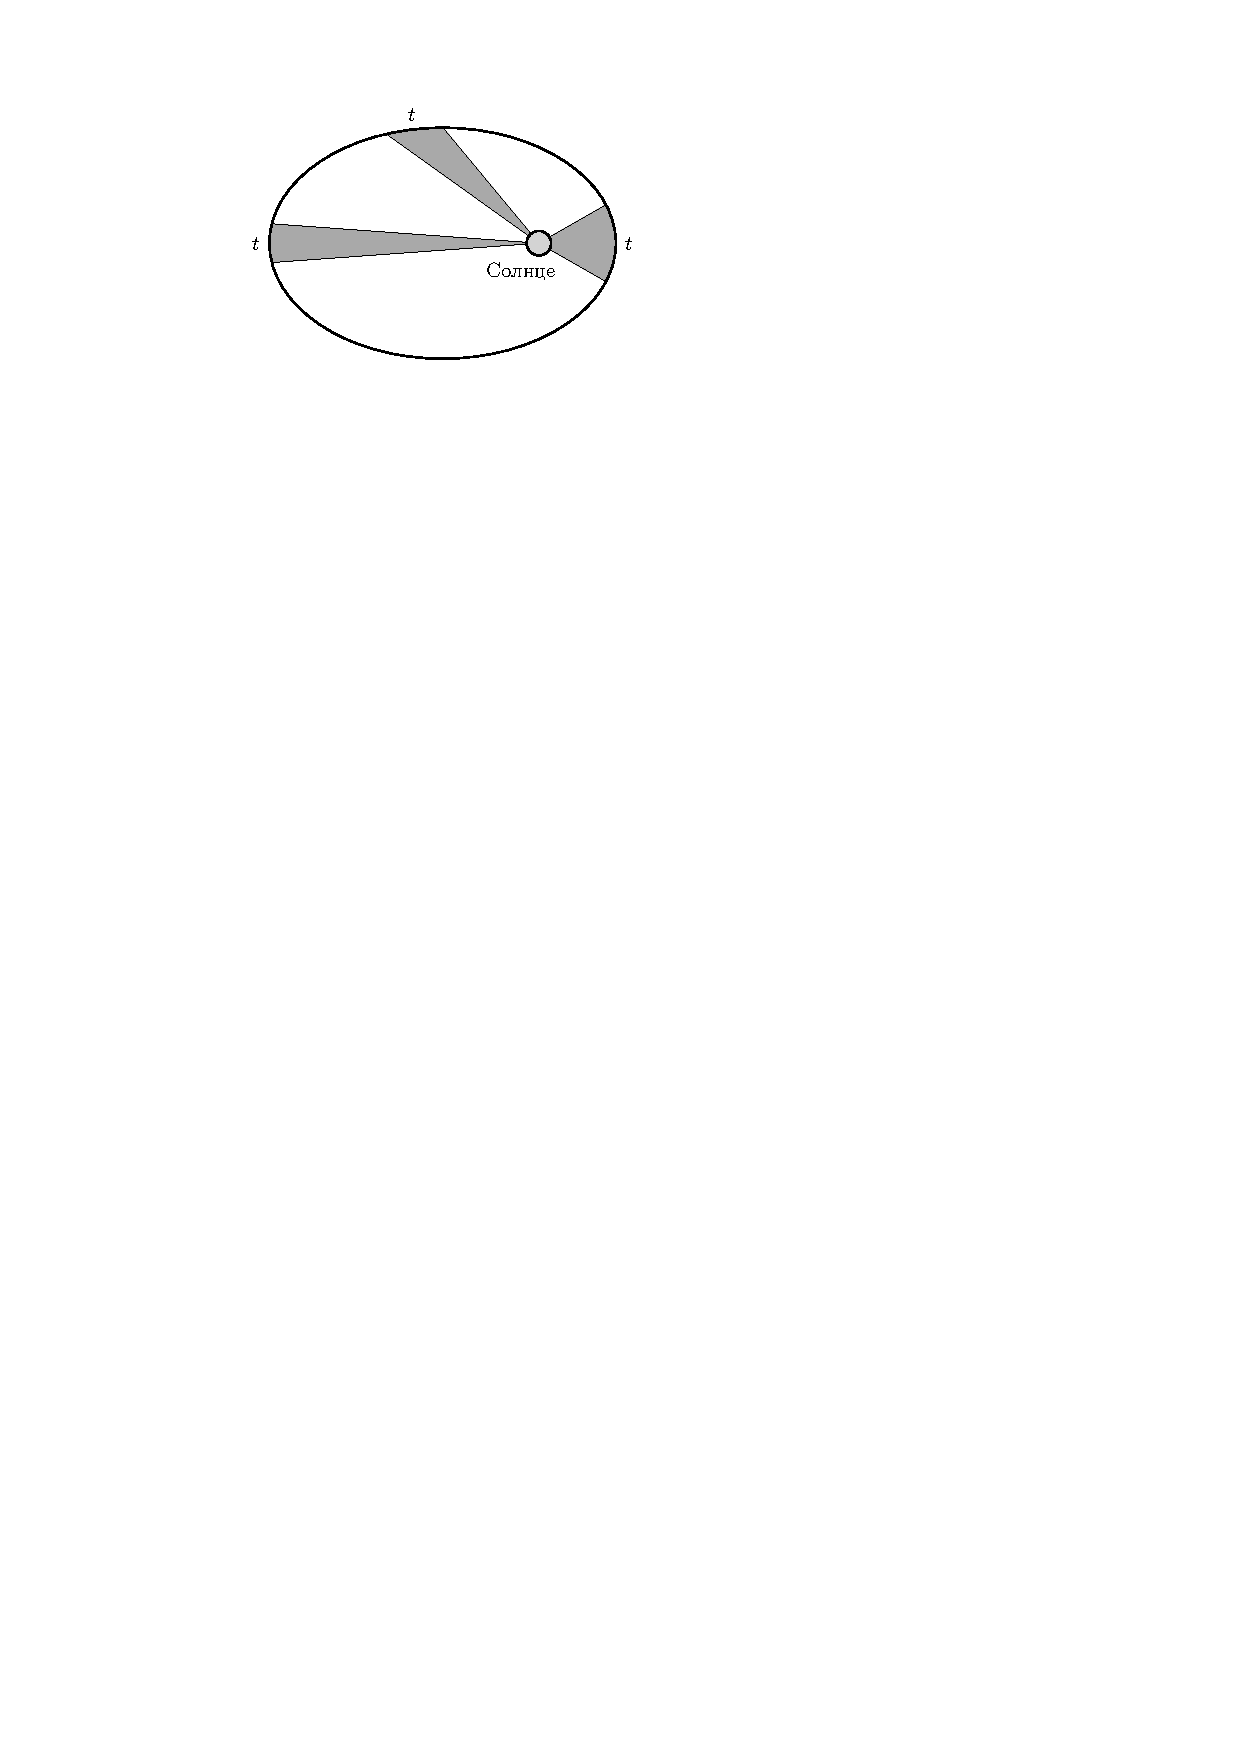
\includegraphics[width = 0.972\textwidth]{second-kepler}
		\caption {Второй закон Кеплера}
	\end{minipage}
\end{figure}

\term{Обобщённый} Ньютоном \term{III-ий закон Кеплера} имеет следующий вид:
\begin{equation}
	\frac{T^2_1( M_1 + m_1)}{T^2_2( M_2 + m_2 )}=\frac{a^3_1}{a^3_2} \quad \Longleftrightarrow \quad
	\frac{T^2 ( M + m )}{a^3} = \frac{4 \pi^2}{G},
\end{equation}
где $M_1$ и $M_2$~--- массы центральных тел, $m_1$ и
$m_2$~--- массы обращающихся вокруг них тел. Так как массы планет
$m$ много меньше массы звезды $M$, $M + m \simeq M$.
